\newpage
\section{Materials and methods}\label{methodology}
This section explains the methodology and the optimization model developed in this work. The section starts with an introduction and overview of the model in Section \ref{met:intro}, followed by a detailed description of the mathematical formulation in Section \ref{met:formulas}. The case study and scenario description is given in Section \ref{met:empirical}. The model validation is described in Section \ref{met:validate} and the open-source programming environment in Section \ref{met:os}

\subsection{Introduction and model overview}\label{met:intro}
This section provides an comprehensive overview of the proposed model. In general, three agents with the following characteristics are considered:
\paragraph{Governance} The governance's main objective is to decarbonizing the residential heating sector. Therefore, the intention is to trigger a heating system change to a sustainable alternative on the multi-apartment building level by financial support for both landlord and tenants. The avowed aim is to find a cost-minimal and socially balanced solution. The financial support can be realized by an investment grant (paid directly from the governance) or rent-charge-related revenues (from the tenants and refunded by the governance) for the landlord and heating costs subsidy payments for the tenants. 
\paragraph{Landlord} is the owner of the multi-apartment building and provides the heating system for the tenants, and is profit-oriented. Thus, a heating system change toward a sustainable alternative only is realized in case of the economic viability of the investment. In this context, the landlord can achieve profitability of the alternative heating system by receiving an investment grant (to reduce the overnight investment costs from the governance) and a rent-charge-related revenue cash flow (from the tenants). 
\paragraph{Tenant} rents a dwelling within the multi-apartment building from the landlord and has rent-related and energy-related spendings. He cannot change the heating system on his authority but depends on the landlord's willingness to realize a low-emission sustainable alternative. Especially in the case of the existing heating system, its costs are directly subject to a higher pricing of CO\textsubscript{2} emissions. Nevertheless, the tenant aims to limit total costs in case of a heating system change at the level of the initial condition.\vspace{0.5cm}

Figure \ref{fig:methodology} shows a sketch illustrating the interrelations between the governance, the landlord, and the tenants. The governance can support the landlord financially by investment grants and by the allowance of rent charge adjustments. At the same time, tenants are supported by a heating costs subsidy payment. The gray bar in the middle indicates that these financial benefits need to be socially balanced and overcome the differences in ownership within the multi-apartment building. The rent or rent charge adjustment is the direct financial exchange between the landlord and the tenant.\vspace{0.5cm}

\begin{figure}[h]
	\centering
	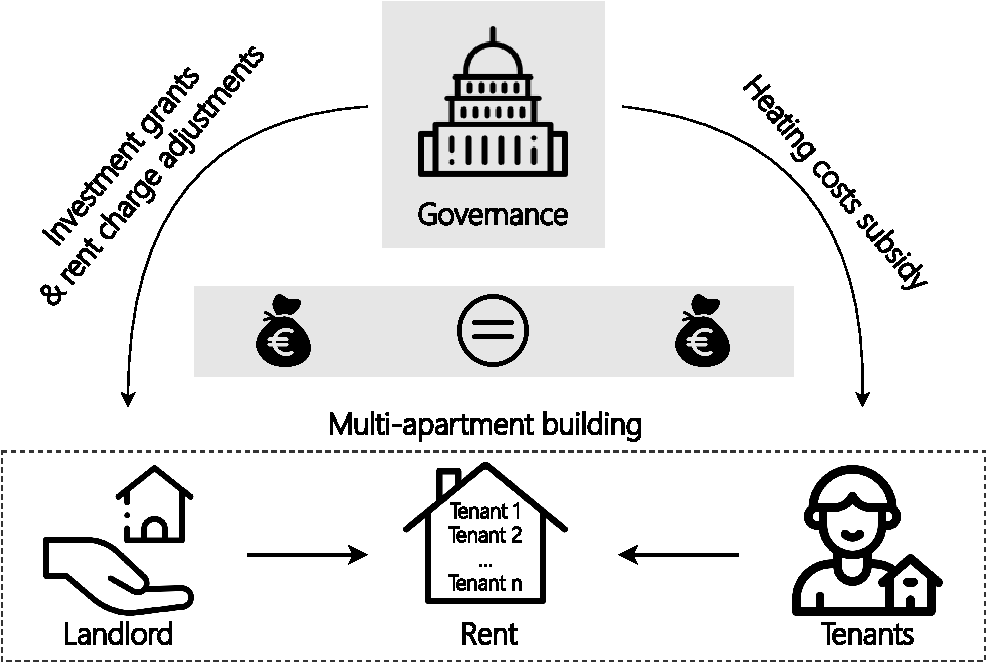
\includegraphics[width=1\linewidth]{figures/3_Methodology/Sketch.pdf}
	\caption{Sketch of the model illustrating the iterrelations between the governance, landlord, and tenants. Financial support from the governance is socially balanced at the multi-apartment building.}
	\label{fig:methodology}
\end{figure}

\subsection{Mathematical formulation of the model}\label{met:formulas}
This section explains the mathematical formulation of the optimization model in detail. First, the objective function is defined. Then, a detailed explanation of the model's constraints is given. 

\subsubsection{Model's objective function}
The objective function of the model is to minimize governance's total costs, including investment grants and subsidy payments\footnote{This corresponds to the maximization of the governance's net present value.}. Therefore, the objective function can be written as follows: 
\begin{align}\label{objective}
\underset{x}{\mathrm{min~}} \Psi + \sum_{y} \sum_{m} \frac{n}{(1+i_g)^y} \cdot \Omega_{y,m}
\end{align}

where $\Psi$ is the investment grant paid tothe landlord and $\Omega_{y,m}$ the heating costs subsidy payment paid to a single tenant in year $y$ and month $m$. In addition, $n$ is the number of tenants\footnote{It is assumed that the multi-apartment building consists of $n$ equal tenants.} and $i_g$ the governance's interest rate. The model's decision variables are included in the decision variable vector $x$. We refer to the nomenclature at the beginning of the paper containing a list of all decision variables.

\subsubsection{Model's constraints}
Equation \ref{c:demand} describes the load satisfaction of the total heat demand within the multi-apartment building using the alternative heating system in each time step (year and month) 
\begin{align}\label{c:demand}
n \cdot d_{y,m} \leq q_{y,m} \quad :\forall y,m
\end{align}

where $d_{y,m}$ is the total heat demand of a tenant's dwelling and $q_{y,m}$ the heat demand covered by the alternative heating system in $y$ and $m$. Building on this, Equation \ref{c:capacity} defines the minimum required newly installed capacity of the heating system alternative
\begin{align}\label{c:capacity}
\alpha_{m} \cdot q_{y,m} \leq \pi \quad :\forall y,m
\end{align}

where $\alpha_{m}$ is the load factor transforming the monthly amount of heat demand to the corresponding peak demand. Equation \ref{c:investment} defines the landlord's overnight investment costs ($\zeta$)
\begin{align}\label{c:investment}
\zeta = \pi \cdot c_{alt} + n \cdot c_{con} - \Psi
\end{align}

where $c_{alt}$ is the specific investment costs of the heating system alternative and $c_{con}$ the construction costs of an dwelling. Equation \ref{c:upper_inv_limit} defines the upper bound for the investment grant 
\begin{align}\label{c:upper_inv_limit}
\Psi \leq \hat{d} + n \cdot c_{con}
\end{align}

where $\hat{d}$ is the peak value of the heat demand. Equation \ref{c:revenues} defines the rent-related revenues of the landlord ($\lambda_{y,m}$)
\begin{align}\label{c:revenues}
\lambda_{y,m} = a \cdot n \cdot (\bar{r} + r_{y,m}) \quad :\forall y,m
\end{align}

where $\bar{r}$ is the initial rent price, $r_{y,m}$ the rent charge adjustment associated with the heating system change in $y$ and $m$ and $a$ the area of a tenant's dwelling. Equation \ref{c:npv} sets the landlord's net present value of the alternative heating system investment equal to zero
\begin{align}\label{c:npv}
-\zeta + \sum_{y} \sum_{m} \frac{1}{(1+i_l)^y} \cdot \lambda_{y,m} = 0
\end{align}

where $i_l$ is the landlord's interest rate. Equation \ref{c:ten1} defines the initial annual spendings of all tenants ($\kappa_{y}$) using the existing heating system 
\begin{align}\label{c:ten1}
\kappa_{y} = n \cdot (\bar{r} \cdot a + \sum_{m} q_{load,y,m} \cdot p_{init,y,m}) \quad :y=y_0
\end{align}

where $p_{init,y,m}$ is the price of the conventional fuel initially supplying the heat demand in $y$ and $m$. Building on this, Equation \ref{c:ten2} sets the tenants' total spendings ($K_{init}$)
\begin{align}\label{c:ten2}
K_{init} = -\sum_{y} \frac{1}{(1+i_{t})^y} \cdot \kappa_{y_0}
\end{align}

where $\sigma_{y_0}$ represents the initial tenants' spendings from Equation \ref{c:ten1} above and $i_t$ the tenant's interest rate. Equation \ref{c:ten3} defines the total spendings of all tenants ($K_{alt}$) realizing the sustainable heating system alternative
\begin{align}\label{c:ten3}
	K_{alt} = -\sum_{y} \sum_{m} \frac{n}{(1+i_{t})^y} \left(a \cdot (\bar{r} + r_{y,m}) + q_{y,m} \cdot p_{alt,y,m}-\Omega_{y,m} \right)
\end{align}

and Equation \ref{c:ten4} defines constant remaining spendings (i.e., economic viability) for the tenants in case of the heating system change.
\begin{align}\label{c:ten4}
K_{alt} = K_{init}
\end{align}

Equation \ref{c:con_sub} defines constant heat costs subsidy payments and Equation \ref{c:con_rent} constant total rent price for a tenant in $y$.
\begin{alignat}{2}
\Omega_{y,m} = \Omega_{y,m-1} \quad &:y\label{c:con_sub}\\
\bar{r} + r_{y,m} = \bar{r} + r_{y,m-1} \quad &:y\label{c:con_rent}
\end{alignat}

Equation \ref{c:temp_rent} allows rent charge adjustment by the landlord only every two years and Equation \ref{c:rent_upper1} and \ref{c:rent_upper2} set a upper bound to the rent charge adjustment
\begin{alignat}{3}
\bar{r} + r_{y,m} = \bar{r} + r_{y-1,m} \quad &:\forall y\backslash \{y_0\},m~\text{if}~y~\text{mod}~2=0\label{c:temp_rent}\\
\bar{r}+r_{y,m} \leq \rho \cdot \bar{r} \quad &:\forall y \in {y_0}\label{c:rent_upper1}\\
\bar{r}+r_{y,m} \leq \rho \cdot \bar{r}+r_{y-1,m} \quad &:\forall y\backslash \{y_0\}\label{c:rent_upper2}
\end{alignat}

by introducing $\rho$, as the rent charge adjustment upper bound. Equation \ref{c:final} defines the financial support parity between the landlord and all tenants at the multi-apartment building level from the governance's perspective 
\begin{align}\label{c:final}
\underbrace{\Psi +  n \cdot \sum_{y} \sum_{m} \frac{r_{y,m}}{(1+i_{g})^y}}_{\text{landlord's financial support}}= \underbrace{n \cdot \sum_{y} \sum_{m} \frac{\Omega_{y,m}}{(1+i_{g})^y}}_{\text{tenants' financial support}}
\end{align}



\subsection{Empirical settings and case study description}\label{met:empirical}
\todo{18.10.2021}

\subsubsection{Description of the multi-apartment building}

\def\checkmark{\tikz\fill[scale=0.4](0,.35) -- (.25,0) -- (1,.7) -- (.25,.15) -- cycle;} 
\definecolor{Gray}{gray}{0.95}
\begin{table}[h]
	\centering
	\setlength{\extrarowheight}{.5em}
	\scalebox{0.85}{
		\begin{tabular}{cccc}
			\toprule
			Scenario  & Climat target & Heat pump & District heating \\\hline
			Low CO\textsubscript{2} price development (LD) & none & \cellcolor{Gray} \checkmark & \cellcolor{Gray} \checkmark\\
			\textit{Gradual Development} (GD) & \SI{2.0}{°C} & \cellcolor{Gray} \checkmark & \cellcolor{Gray} \checkmark\\
			\textit{Societal Commitment} (SC) & \SI{1.5}{°C} & \cellcolor{Gray} \checkmark & -\\
			\textit{Directed Transition} (DT) & \SI{1.5}{°C} & - & \cellcolor{Gray} \checkmark\\ 
			\bottomrule
	\end{tabular}}
	\caption{}
	\label{tab:scenarios}
\end{table}

% TODO: Revelant empirical data 

% TODO Interest rate: 3 (governance),5 (tenants), 7 (landlord) percentage; inflation

\subsubsection{Scenario description}


\subsection{Validation of the model}\label{met:validate}
This section aims to test the presented model and its functionalities. However, a model validation using existing empirical data can not be applied in this case. There is simply a lack of comparable data from real cases. Therefore, a small illustrative case study is chosen to demonstrate the main functionalities and to verify the model. We assume a single landlord and tenant in a representative single-family household implementing a heat pump. It is assumed that the landlord's and tenant's interest rate is equal (\SI{3}{\%}). A detailed description of the empirical settings can be found in \ref{app:verify}. Figure \ref{val:npv} shows the landlord's (a) and tenant's (b) net present value. 

\begin{figure}[h]
	\begin{subfigure}[c]{0.5\textwidth}
		\centering
		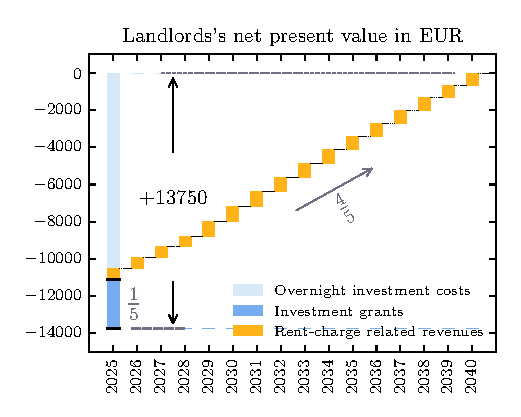
\includegraphics[width=1\linewidth]{figures/3_Methodology/Validate-Landlord.eps}
		\subcaption{Development of landlord's net present value}
		\label{fig:landlord}
	\end{subfigure}
	\begin{subfigure}[c]{0.5\textwidth}
		\centering
		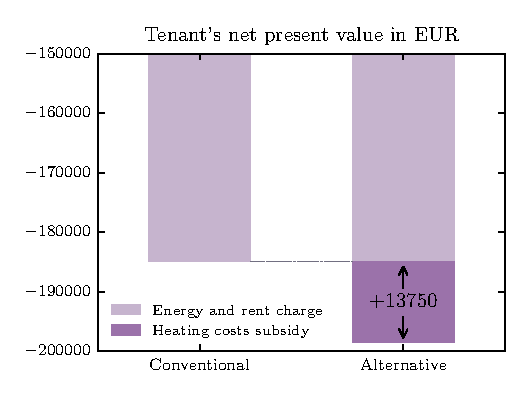
\includegraphics[width=1\linewidth]{figures/3_Methodology/Validate-Tenant.eps}
		\subcaption{Comparison of tenant's net present value}
		\label{fig:tenant}
	\end{subfigure}
	\caption{Landlord's and tenant's net present value and equal financial support. The landlord reaches a net present value equal to zero in 2040 resulting from an investment grant and rent-charge related revenues. The tenant's net present value remains constant compared to the conventional heating system resulting from heating costs subsidy payments.}
	\label{val:npv}
\end{figure}

Both agents receive equal financial support with a total of \SI{13750}{EUR}. One finfth of the landlord's support is paid as an investment grant and four-fifths as rent-charge related revenues. The tenant receives a heating costs subsidy. The level of financial support results exactly in (i) a landlord's net present value equal to zero within the time horizon of 15 years (see Figure \ref{fig:landlord}) and (ii) a constant remaining net present value of tenant compared to the conventional (existing) heating system (including the initial rent charge) (see Figure \ref{fig:tenant}). 

\subsection{Open-source programming environment and data format}\label{met:os}
The developed optimization model is implemented in Python using the modeling framework Pyomo \cite{hart2017optimization}. It is solved with the solver Gurobi version 9.0.3. We use for data analysis the common data format template developed by the Integrated Assessment Modeling Consortium (IAMC) using the open-source Python package pyam \cite{huppmann2021pyam}. Note that all materials used in this study are disclosed as part of the publication at GitHub \footnote{https://github.com/sebastianzwickl}. We refer to the repository for the codebase, data collection, and further information. 